\documentclass[12pt,letterpaper]{article}
\usepackage[utf8]{inputenc}
\usepackage[spanish]{babel}
\usepackage{amsmath}
\usepackage{amsfonts}
\usepackage{amssymb}
\usepackage{graphicx}
\usepackage{ragged2e}
\usepackage{cite}
\usepackage{float}
\usepackage{wasysym}
\usepackage{subfig}
\graphicspath{ {imagenes/} }
\usepackage{amsmath, amsfonts, amssymb}
\usepackage[left=2.5cm,right=2.5cm,top=2cm,bottom=2cm]{geometry}
\author{Javier Said Naranjo Miranda\\ Grupo: 2CM4}
\title{Teoría Computacional\\ B\'usqueda de texto}
\begin{document}
\maketitle
\justify
A continuación se mostrara la tabla de transiciones del aut\'omata no deterministico para la b\'usqueda de texto, en este caso sera para la b\'usqueda de la palabra \textit{web} y de \textit{ebay} .\\
Se define el caracter $\sum $ como el conjunto de todos los caracteres ASCII imprimibles, distintos de \textit{w},  \textit{e}, \textit{b}, \textit{a}, \textit{y}.\\
\begin{center}
\begin{tabular}{| c || c | c | c | c | c | c |} \hline
 & $ \sum $ & w & e & b & a & y \\
\hline\hline
$\phi$ & $\phi$ & $\phi$ & $\phi$ & $\phi$ & $\phi$ & $\phi$ \\
\hline
$\rightarrow$ $\lbrace q0 \rbrace$ & $\lbrace q0 \rbrace$ & $\lbrace q0, q1 \rbrace$ & $\lbrace q0, q4 \rbrace$ & $\lbrace q0 \rbrace$ & $\lbrace q0 \rbrace$ & $\lbrace q0 \rbrace$ \\
\hline
$\lbrace q0, q1 \rbrace$ & $\lbrace q0 \rbrace$ & $\lbrace q0, q1 \rbrace$ & $\lbrace q0, q2, q4 \rbrace$ & $\lbrace q0 \rbrace$ & $\lbrace q0 \rbrace$ & $\lbrace q0 \rbrace$ \\
\hline
$\lbrace q0, q4 \rbrace$ & $\lbrace q0 \rbrace$ & $\lbrace q0, q1 \rbrace$ & $\lbrace q0, q4 \rbrace$ & $\lbrace q0, q5 \rbrace$ & $\lbrace q0 \rbrace$ & $\lbrace q0 \rbrace$ \\
\hline
$\lbrace q0, q5 \rbrace$ & $\lbrace q0 \rbrace$ & $\lbrace q0, q1 \rbrace$ & $\lbrace q0, q4 \rbrace$ & $\lbrace q0 \rbrace$ & $\lbrace q0, q6 \rbrace$ & $\lbrace q0 \rbrace$ \\
\hline
$\lbrace q0, q6 \rbrace$ & $\lbrace q0 \rbrace$ & $\lbrace q0, q1 \rbrace$ & $\lbrace q0, q4 \rbrace$ & $\lbrace q0 \rbrace$ & $\lbrace q0 \rbrace$ & $\lbrace q0, q7 \rbrace$ \\
\hline
$*\lbrace q0, q7 \rbrace$ & $\lbrace q0 \rbrace$ & $\lbrace q0, q1 \rbrace$ & $\lbrace q0, q4 \rbrace$ & $\lbrace q0 \rbrace$ & $\lbrace q0 \rbrace$ & $\lbrace q0 \rbrace$ \\
\hline
$\lbrace q0, q2, q4 \rbrace$ & $\lbrace q0 \rbrace$ & $\lbrace q0, q1 \rbrace$ & $\lbrace q0, q4 \rbrace$ & $\lbrace q0, q3, q5 \rbrace$ & $\lbrace q0 \rbrace$ & $\lbrace q0 \rbrace$ \\
\hline
$*\lbrace q0, q3, q5 \rbrace$ & $\lbrace q0 \rbrace$ & $\lbrace q0, q1 \rbrace$ & $\lbrace q0, q4 \rbrace$ & $\lbrace q0 \rbrace$ & $\lbrace q0, q6 \rbrace$ & $\lbrace q0 \rbrace$ \\
\hline
     
\end{tabular}
%\caption{Tabla de transiciones del aut\'omata no determinista.}
\end{center}
\justify
Para hacer la equivalencia entre el aut\'omata finito determinista y el no determinista, es necesario hacer la construcci\'on de los subconjuntos del conjunto de estados.\\
A continuaci\'on se muestra el etiquetado de cada uno de los subconjuntos.\\
\begin{center}
\begin{tabular}{| c | c |} \hline
Subconjunto & Etiqueta \\
\hline\hline
$\phi$ & \textit{A} \\
\hline
$\lbrace q0 \rbrace$ & \textit{B}  \\
\hline
$\lbrace q0, q1 \rbrace$ & \textit{C} \\
\hline
$\lbrace q0, q4 \rbrace$ & \textit{D} \\
\hline
$\lbrace q0, q5 \rbrace$ & \textit{E} \\
\hline
$\lbrace q0, q6 \rbrace$ & \textit{F} \\
\hline
$\lbrace q0, q7 \rbrace$ & \textit{G} \\
\hline
$\lbrace q0, q2, q4 \rbrace$ & \textit{H} \\
\hline
$\lbrace q0, q3, q5 \rbrace$ & \textit{I} \\
\hline
     
\end{tabular}
\end{center}
\newpage
A continuaci\'on se muestra la tabla de transiciones del aut\'omata no determinista con el reetiquetado correspondiente. De esta manera obtenemos la equivalencia entre el AFN y el AFD.\\

\begin{center}
\begin{tabular}{| c || c | c | c | c | c | c |} \hline
 & $ \sum $ & w & e & b & a & y \\
\hline\hline
\textit{A} & \textit{A} & \textit{A} & \textit{A} & \textit{A} & \textit{A} & \textit{A} \\
\hline
$\rightarrow$ \textit{B} & \textit{B} & \textit{C} & \textit{D} & \textit{B} & \textit{B} & \textit{B} \\
\hline
\textit{C} & \textit{B} & \textit{C} & \textit{H} & \textit{B} & \textit{B} & \textit{B} \\
\hline
\textit{D} & \textit{B} & \textit{C} & \textit{D} & \textit{E} & \textit{B} & \textit{B} \\
\hline
\textit{E} & \textit{B} & \textit{C} & \textit{D} & \textit{B} & \textit{F} & \textit{B} \\
\hline
\textit{F} & \textit{B} & \textit{C} & \textit{D} & \textit{B} & \textit{B} & \textit{G} \\
\hline
*\textit{G} & \textit{B} & \textit{C} & \textit{D} & \textit{B} & \textit{B} & \textit{B} \\
\hline
\textit{H} & \textit{B} & \textit{C} & \textit{D} & \textit{I} & \textit{B} & \textit{B} \\
\hline
*\textit{I} & \textit{B} & \textit{C} & \textit{D} & \textit{B} & \textit{F} & \textit{B} \\
\hline
     
\end{tabular}
\end{center}
\justify
A continuaci\'on se muestra una imagen del diagrama del aut\'omata determinista para la b\'usqueda de las palabras \textit{web} y \textit{ebay}.\\

\begin{figure}[H]
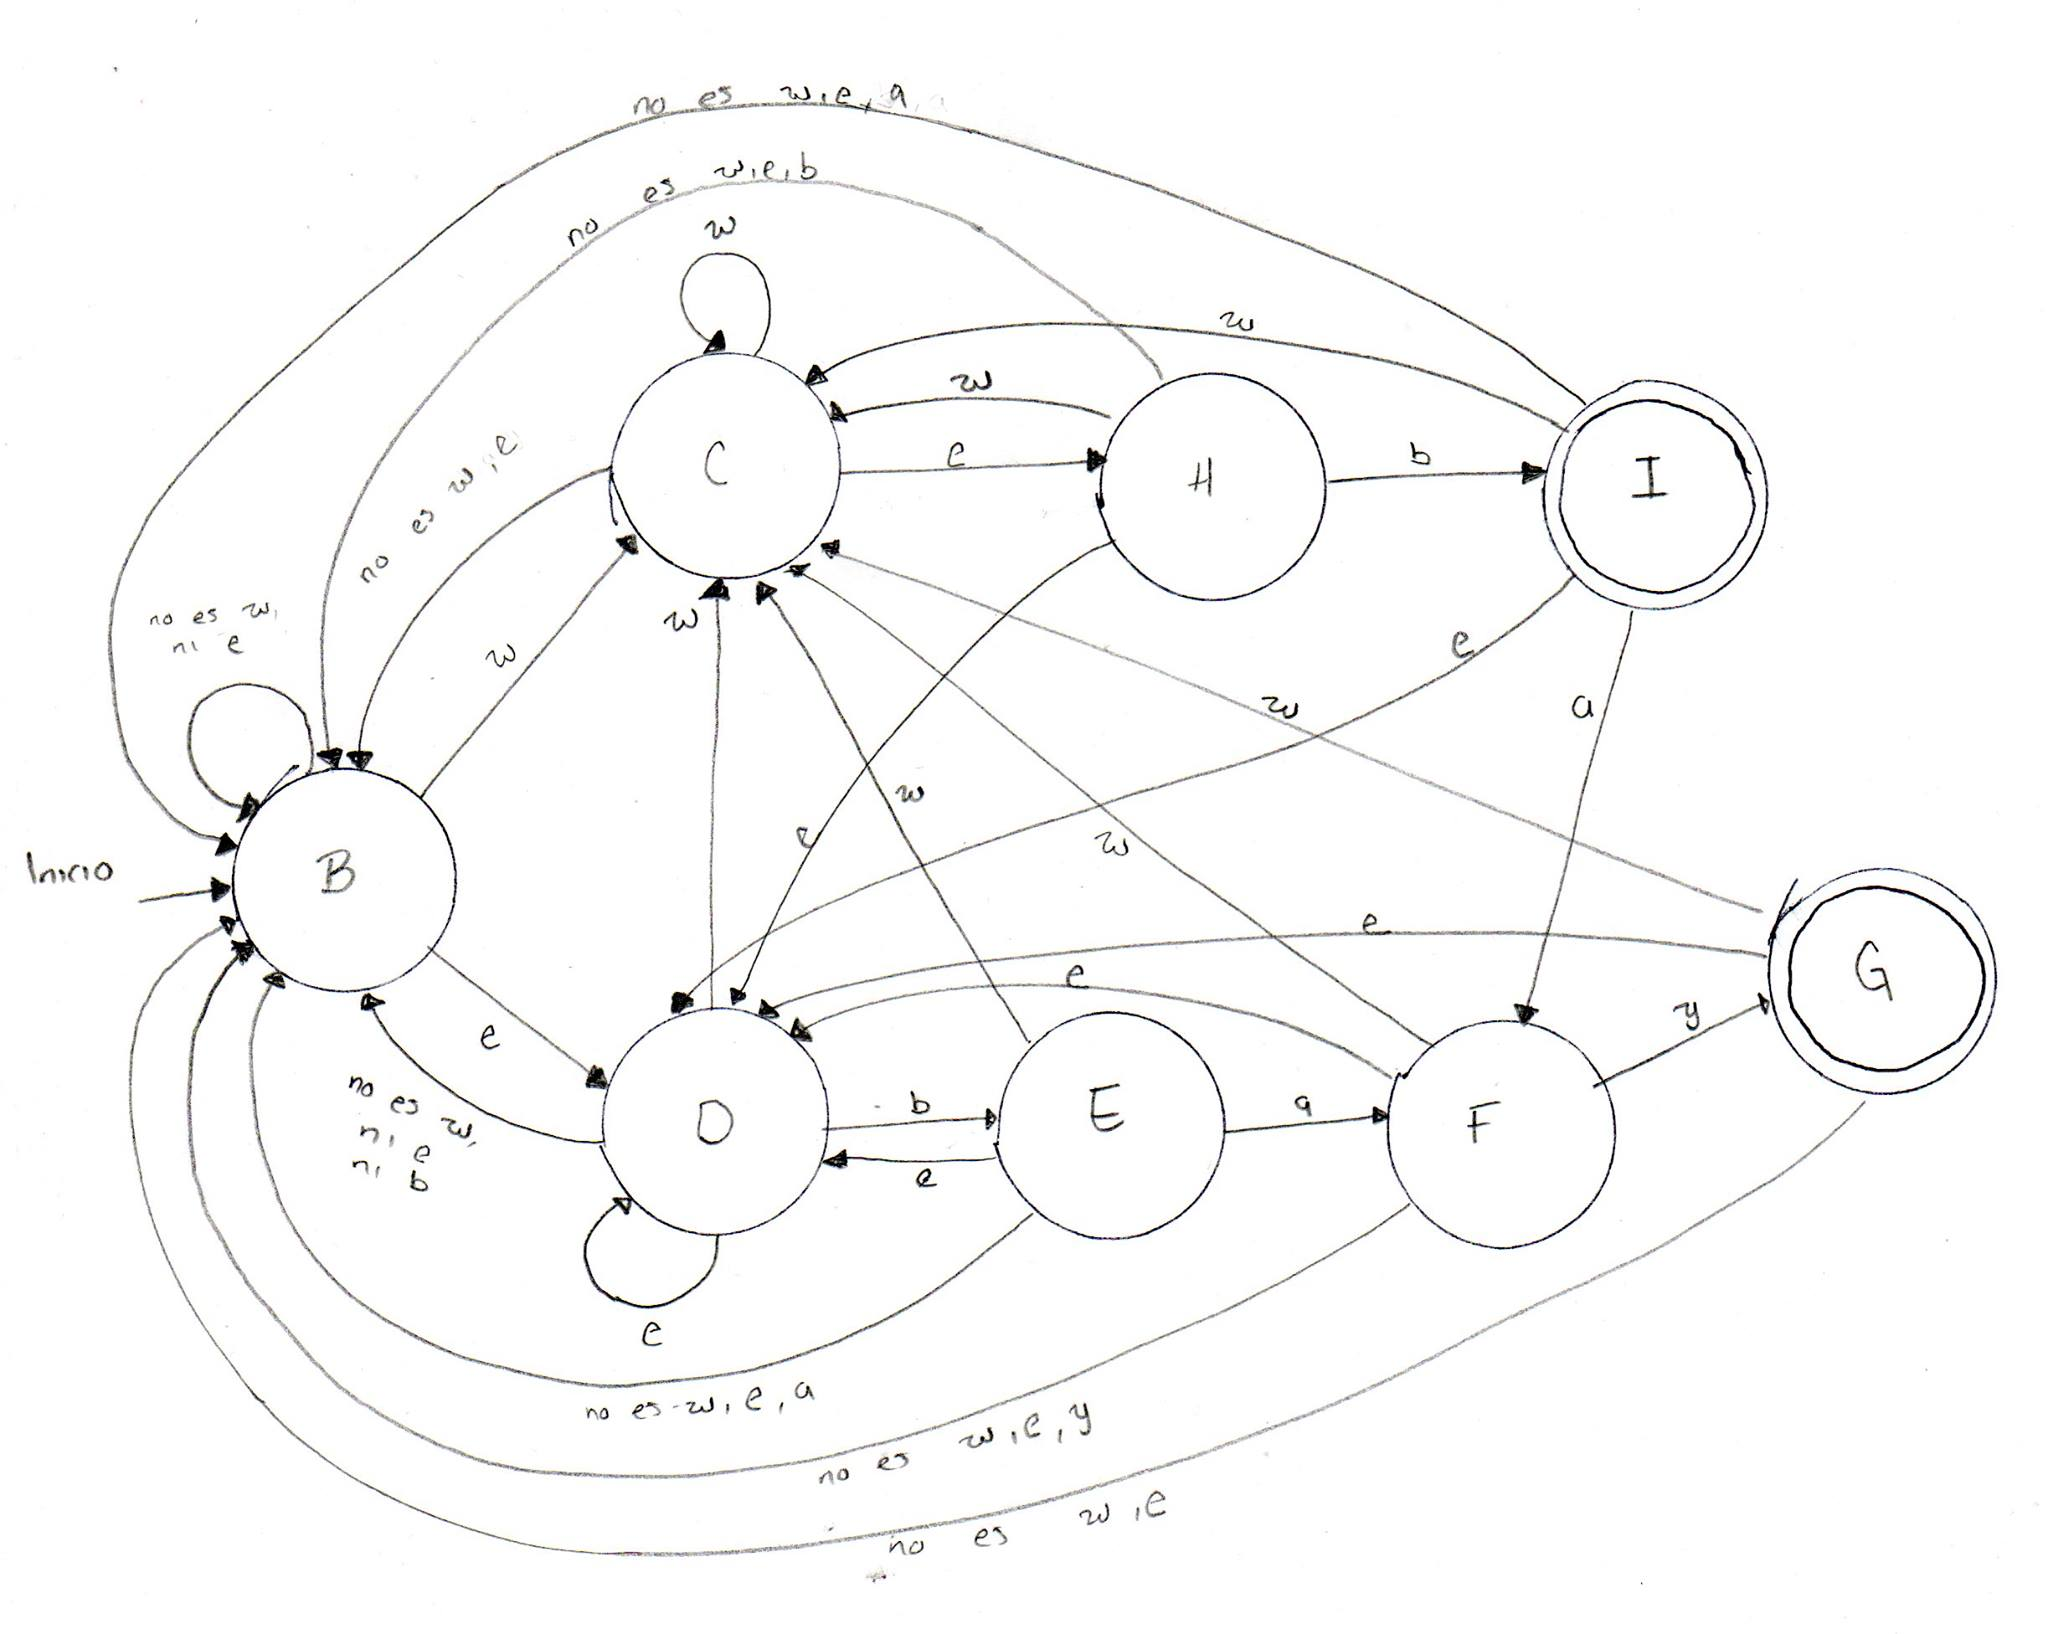
\includegraphics[width=\textwidth, height=10cm]{busqueda.jpg}
\label{fig: busqueda}
\caption{Diagrama del aut\'omata determinista}
\end{figure}
\begin{thebibliography}{X}
\bibitem{Dan} \textsc{	HOPCROFT JOHN, MOTWANI RAJEEV},
<<Introduction to Automata Theory,
Languages and Computation>>,
\textit{Addison Wesley},2008
\end{thebibliography}
\end{document}